\documentclass{assignment}
\ProjectInfos{在生活中感知材料的魅力}{GENS1004}{2020-2021学年第一学期}{第一次作业}{大自然给电池研究带来的灵感}{陈稼霖}{45875852}
\begin{document}
\begin{ti}
    什么是电池?列举2种典型的电池体系并描述其原理。
\end{ti}
\begin{da}
    电池指的是将本身储存的化学能转化成电能的装置,其一般由正极、负极和电解质构成,当接通正负两极,电池中发生电化学反应而将化学能转化为电能。

    \textbf{丹尼尔电池}(又称锌铜原电池),如图\ref{Daniell}所示,将锌置于\ce{ZnSO4}溶液中作为负极,铜置于\ce{CuSO4}溶液中作为正极,并用盐桥或离子膜连接两种电解质溶液,当正负极接通,发生如下反应:
    \begin{center}
        负极:\ce{Zn -> Zn^{2+} + 2e^-},\\
        正极:\ce{Cu^{2+} + 2e^- -> Cu},
    \end{center}
    从而产生电流。丹尼尔电池是一次性电池,无法重复充放电使用。
    \begin{figure}[h]
        \centering
        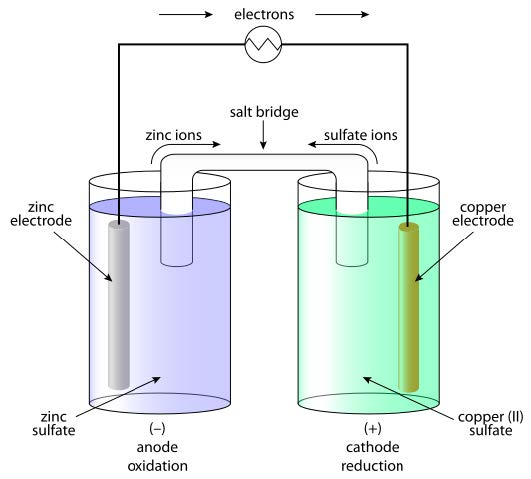
\includegraphics[width=.25\columnwidth]{DaniellBattery.jpg}
        \caption{丹尼尔电池}
        \label{Daniell}
    \end{figure}

    \textbf{铅酸蓄电池},如图\ref{Lead-acid},以铅为负极,以\ce{PbO2}为正极,置入硫酸溶液中。放电时,发生如下反应:
    \begin{center}
        负极:\ce{Pb + SO_4^{2-} -> PbSO_4 + 2e^-},\\
        正极:\ce{PbO_2 + 4H^+ + SO_4^{2-} + 2e^- -> PbSO_4 + 2H_2O + 2e^-},
    \end{center}
    从而产生电流。铅酸蓄电池可以重复充放电,当向阳极(负极)施加比阴极(正极)更高的电势,发生如下反应:
    \begin{center}
        阳极(负极):\ce{PbSO_4 + 2e^- -> Pb + SO_4^{2-}},\\
        阴极(正极):\ce{PbSO_4 + 2H_2O -> PbO_2 + 4H^+ + SO_4^{2-}},
    \end{center}
    从而使正极、负极和电解质重新回到原有的状态,将电能转化为化学能储存起来。
    \begin{figure}[h]
        \centering
        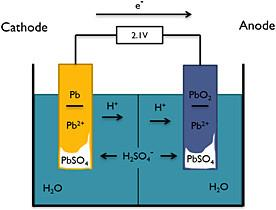
\includegraphics[width=.25\columnwidth]{Lead-acidBattery.jpg}
        \caption{铅酸蓄电池}
        \label{Lead-acid}
    \end{figure}
\end{da}

\begin{ti}
    有哪些主要的碳材料,石墨烯的主要特点是什么?有哪些主要的应用?
\end{ti}
\begin{da}
    碳材料主要分为四类:
    \begin{itemize}
        \item[(1)] 传统碳材料,如木炭、竹炭、活性炭、炭黑、焦炭、天然石墨等;
        \item[(2)] 特种碳材料,如金刚石、碳纤维、碳分子筛、柔性石墨、氟化石墨;
        \item[(3)] 纳米碳材料,如富勒烯、碳纳米管、纳米金刚石、石墨烯等;
        \item[(4)] 新型碳材料:如课堂上介绍的葡萄藤状的自组装碳纳米管材料、以螃蟹壳为模板的具有扭曲胶合的中空纳米阵列结构的碳材料、火龙果状结构的介孔碳、石榴状结构的空心团簇组成的碳材料、人体肠道绒毛状的碳纤维、碳化的天然木材。
    \end{itemize}

    石墨烯是一种由单层碳原子以sp$^2$杂化轨道组成六角形蜂窝状结构的二维碳材料,其主要特点有:
    \begin{itemize}
        \item[(1)] 良好的强度和韧性:石墨烯的理论杨氏模量达$1.0$ TPa,固有的拉伸强度为$130$ GPa;
        \item[(2)] 良好的导电性:石墨烯具有sp$^2$杂化形成的大$\pi$键,在常温下的载流子迁移率达$15000$ cm$^2$/(V$\cdot$s);
        \item[(3)] 良好的导热性:石墨烯的导热系数达$5300$ W/mK;
        \item[(4)] 良好的吸附能力:作为一种单层二维材料,石墨烯的比表面很大,故可以吸附很多的各种原子和分子;
        \item[(5)] 良好的光学特性:石墨烯在很宽的波长范围内几乎是透明的;
        \item[(6)] 超疏水性和超亲油性:石墨烯在非极性溶剂中表现出良好的溶解性。
    \end{itemize}

    石墨烯具有广泛的应用,例如:
    \begin{itemize}
        \item[(1)] 电池电极:课堂上提到过,由于石墨烯良好的吸附能力,石墨烯可以用来负载金属锂从而作为锂离子电池的电极;
        \item[(2)] 导电剂:由于石墨烯良好的导电性能,加入石墨烯可以增加介质的导电性能;
        \item[(3)] 单分子气体侦测:由于石墨烯良好的吸附性能以及很大的比表面积,可以通过石墨烯吸附气体分子时的局域电阻变化,侦测气体;
        \item[(4)] 集成电路:作为单层材料,在表面积一定的情况下,石墨烯质量和体积都很小,且具有良好的导电性,故可以用来制作集成电路;
        \item[(5)] 导热材料:石墨烯很薄且导热性很好,适合作为导热材料;
        \item[(6)] 科学研究:石墨烯是一种相对简单的、却又有奇特性质(如上面所述的主要特点,能带中的狄拉克锥以及反常量子霍尔效应等)的二维材料,是材料科学、凝聚态物理研究的热点。
    \end{itemize}
\end{da}
\end{document}